\documentclass[aspectratio=169,11pt,hyperref={colorlinks=true}]{beamer}
\usepackage[utf8]{inputenc}
\usepackage[T1]{fontenc}
\usepackage{fontspec}
\usepackage[absolute,overlay]{textpos}
\usepackage{listingsutf8}
\usepackage{listings-golang}
\usepackage{tikz}
\usepackage{color}
\usepackage{fontawesome5}
\usepackage{svg}

% \setbeameroption{show notes}


\title{Tekton Project Update and Roadmap \faRobot\faCat}
\date[9 May 2023 ]{cdCon + GitOpsCon | 9 May 2023 | \faTwitter ~@tektoncd | \faGithub ~tektoncd}
\author[Andrea Frittoli]{%
  Andrea Frittoli \\
  Open Source Advocate \\
  andrea.frittoli@uk.ibm.com
}

\usetheme{af}

% Code style
\setlststyle

\lstdefinelanguage{koyaml}{
  keywords={github, com, afrittoli, examples, ms, go, helloworld},
  sensitive=false,
  comment=[l]{\#},
  morestring=[b]',
  morestring=[b]"
}

% Automatic section frame
% \AtBeginSection{\frame{\sectionpage}}

\begin{document}

\begin{frame}
\titlepage{}
\end{frame}

\begin{speakerframe}[af_wind.jpg]{Andrea Frittoli}%
  {%
  \faGithub ~afrittoli | \faLinkedin ~andreafrittoli | \faTwitter ~@blackchip76
  }%
  {%
  \begin{itemize}
    \item{Open Source Advocate @ IBM}
    \item{Lives in Wales, enjoys the wind}
    \item{Tekton maintainer, Governing Board}
    \item{CDEvents maintainer, Events SIG co-chair}
    \item{CDF Technical Oversight Committee \\ Governing Board}
  \end{itemize}
  }%
\end{speakerframe}

\begin{lpicrblack}[chewy-I-rgDPLKogs-unsplash.jpg]{%
  Photo by \href{https://unsplash.com/@chewy}{\underline{Chewy}}, CC0
  }%
  {%
  \tableofcontents
  }%
  {}
  \frametitle{Agenda}
\end{lpicrblack}

\section[Introduction]{Introduction}

\begin{sectionwithpic}[mike-benna-X-NAMq6uP3Q-unsplash.jpg]{Photo by \href{https://unsplash.com/@mbenna}{\underline{Mike Benna}}, CC0}
\end{sectionwithpic}

\begin{stripedframe}%
  {%
  Tekton is an open-source framework \\ for creating CI/CD systems \\ ~
  }%
  {%
  Cloud Native \\
  \vspace{0.03\textheight}
  Serveless, Scalable Pipelines \\
  \vspace{0.03\textheight}
  Security Oriented \\
  \vspace{0.03\textheight}
  SLSA Compliant Pipelines
  }%
  {%
  Standardization \\
  \vspace{0.03\textheight}
  Built In Best Practices \\
  \vspace{0.03\textheight}
  Maximum Flexibility \\
  }%
  {%
  \vspace{0.01\textheight}
  Core:
  \begin{itemize}
    \item Pipeline
    \item Triggers
    \item Chains
  \end{itemize}
  ~ \\
  Tools:
  \begin{itemize}
    \item CLI, Dashboard
    \item Operator
  \end{itemize}
  }%
  {%
  Authoring:
  \begin{itemize}
    \item Catalog, Hub
    \item ArtifactHub
  \end{itemize}
  ~ \\
  Add-ons:
  \begin{itemize}
    \item Results
    \item Workflows
  \end{itemize}
  }%
  % \begin{textblock*}{0.13\paperwidth}(0.73\paperwidth,0.65\paperheight)
  %   \includesvg[width=0.13\paperwidth]{img/tekton-icon-color.svg}
  % \end{textblock*}
  % A brief into to Tekton
\end{stripedframe}

\note{
  Tekton is an open-source framework for creating continuous delivery systems (aka CI/CD).
  Tekton is built on top of Kubernetes, and it brings all the cloud-native
  advantages into the CD space: serverless execution, scalability and integration with
  the impressive ecosystem of cloud native tools for logging, monitoring, policy enforcement
  and more.

  Tekton has a very small footprint, which makes it easy to get started with it in your minikube
  or kind cluster. That also means having a small control plan overhead when running
  hundres of pipelines. Tekton particuarly shines in large scale CD environments, as it gives
  DevOps architects the full flexibility they need to setup up a CD system which meets the
  enterprise needs for security and compliance, while letting software engineers quickly and
  easily develop their pipelines through a catalog of curated bulding blocks.

  Tekton benefits from a lively community, with contributions from more than 150 companies
  and a collection of different projects that provide from workflow definition, event handling,
  user interfaces, catalog and security.
}

\begin{lgrayrwhiteframe}
  \frametitle{At a Glance}
  \begin{itemize}
    \item 2018 Initial concept
    \item 2019 Donated to CD Foundation
    \item 2022 Graduated Project
    \begin{itemize}
      \item LTS Releases
      \item Adoptions
      \item Best Practices
      \item Security
    \end{itemize}
  \end{itemize}
  ~
  \begin{itemize}
    \item 150+ Companies
    \item Google, IBM, RedHat, VMWare \& others
  \end{itemize}
  \begin{textblock*}{0.51\paperwidth}(0.57\paperwidth,0.33\paperheight)
    \includesvg[width=0.3\paperwidth]{img/cdf-stacked-color.svg}
  \end{textblock*}
\end{lgrayrwhiteframe}

\begin{lgrayrwhiteframe}
  \frametitle{Defining Pipelines}
  \begin{itemize}
    \item Extend the k8s API with CRDs
    \item Definitions: Task, Pipeline
    \item Execution: TaskRun, PipelineRun
    \item Bindings: \\Workspaces, Parameters, Results
  \end{itemize}
  ~
  \begin{itemize}
    \item TaskRun -> Pod
    \item Step -> Container
    \item Workspace -> Volume, Configmap, Secret
  \end{itemize}
  \begin{textblock*}{0.51\paperwidth}(0.48\paperwidth,0.33\paperheight)
    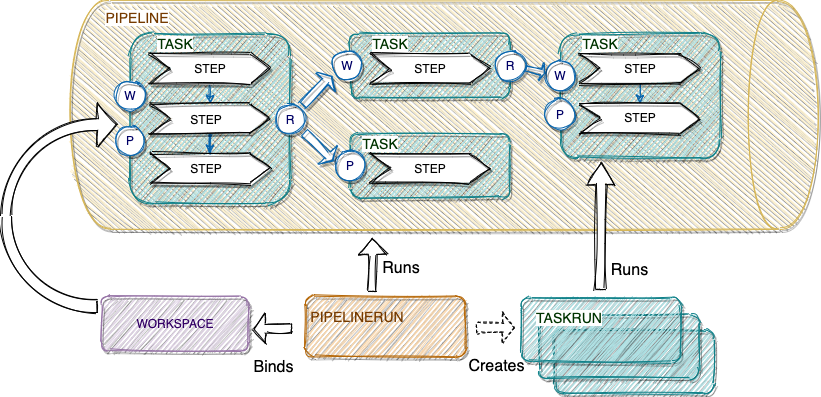
\includegraphics[width=0.5\paperwidth]{img/tekton-workspaces.png}
  \end{textblock*}
\end{lgrayrwhiteframe}

\begin{lgrayframerpic}[pouncing-cat.png]{Public domain photo, CC0}%
  {%
  \begin{itemize}
    \item Tekton Triggers
    \item Webhooks, Events
    \item Filter on branch
    \item Filter on any payload content
    \item Start a pipeline execution
  \end{itemize}
  }%
  {0.30}
  \frametitle{Launching Pipelines}
\end{lgrayframerpic}

\begin{2columnsframe}{Securing Pipelines}%
  {%
  Tekton Chains
  \begin{itemize}
    \item Artifact signing
    \item Artifact provenance
    \item Sigstore integration
  \end{itemize}
  ~\\
  ~\\
  ~\\
  Tekton Pipelines
  \begin{itemize}
    \item Trusted Resources (alpha)
    \item Non-falsifiable Provenance (alpha)
    \item Hermetic Builds (alpha)
    \item Working towards SLSA lvl3
  \end{itemize}
  }{%
  Some chains diagram here
  }
\end{2columnsframe}

\section[What's New]{What's New in Tekton}
\begin{sectionwithpic}[cat-walking-on-stairs.jpg]{Public domain photo, CC0}
\end{sectionwithpic}

\begin{blackframe}
  \frametitle{New pipeline features}
  \begin{itemize}
    \item Two LTS releases v0.44 and v0.47
    \item Remote resolution to beta, config source
    \item Propagation to beta
    \item Custom Task to beta
    \item Array and Object Params and Results to beta
    \item Trusted Resources as alpha
    \item Larger Results via sidecar log as alpha
    \item Artifact Hub support
    \item Env variables in pod template
    \item Distributed tracing for pipelines
    \item Pipeline v1 API (v1beta1 stored by default)
    \item Explicit params combinations in matrix
  \end{itemize}
\end{blackframe}

\begin{blackframe}
  \frametitle{Removed pipeline features}
  \begin{itemize}
    \item Pipeline Resources
    \item Embedded Status
  \end{itemize}
\end{blackframe}

\begin{blackframe}
  \frametitle{Non-pipeline features}
  \begin{itemize}
    \item Scheduled Runs
    \item Chains v1.0
  \end{itemize}
\end{blackframe}

\section[Roadmap]{Roadmap \faRobot\faCat}
\begin{sectionwithpicrx}[julie_falk_flickr_22258190324_6a583208ae_k.png]{Photo by \href{https://www.flickr.com/photos/piper/}{\underline{Julie Falk}}, CC BY-NC 2.0}
\end{sectionwithpicrx}

\begin{blackframe}
  \frametitle{What's coming in Pipeline}
  \begin{itemize}
    \item Pipeline v1.0
    \item Planned LTS patch releases
    \item Artifacts
    \item Non falsifiable provenance
    \item Multiple deployments per cluster
    \item Better tracing
    \item Conformance policy
    \item Dedicated events controller, CDEvents
  \end{itemize}
\end{blackframe}

\begin{blackframe}
  \frametitle{What's coming}
  \begin{itemize}
    \item Chains v1.0
    \item Refreshed catalog
    \item Scheduled Runs
    \item Concurrency controller
    \item Tekton Results
  \end{itemize}
\end{blackframe}

\begin{2columnsframe}{Roadmap \& Vision}%
  {%
  Mission:
  \begin{itemize}
    \item Be the industry-standard,\\
          cloud-native CI/CD platform \\
          components and ecosystems \\
  \end{itemize}
  ~\\
  ~\\
  \tiny~\\
  \normalsize
  Vision:
  \begin{itemize}
    \item Tekton API conformance across\\
          as many CI/CD platforms as possible
  \end{itemize}
  }{%
  Vision:
  \begin{itemize}
    \item A rich catalog of high quality,\\
          reusable Tasks which work\\
          with Tekton conformant systems\\
  \end{itemize}
  ~\\
  ~\\
  \tiny~\\
  \normalsize
  Roadmap 2023:
  \begin{itemize}
    \item Tekton V1 API
    \item Security Features
    \item Observability
    \item Workflows
    \item User stories, Documentation
  \end{itemize}
  }
\end{2columnsframe}

\section[Q\&A]{Thank You! \\Questions?}

\begin{sectionwithpiclargecentral}[carl-jorgensen-5nrnxx_tWe8-unsplash.jpg]{Brecon Beacons, Walse, Photo by \href{https://unsplash.com/@scamartist}{\underline{Carl Jorgensen}}, CC0}
\end{sectionwithpiclargecentral}

\begin{blackframe}
  \frametitle{References}
  \begin{itemize}
    \item \large Come and Join Us at Tekton!
    \item \normalsize Tekton community: \href{https://github.com/tektoncd/community}{github.com/tektoncd/community} \\
  \end{itemize}
  \begin{itemize}
    \item Slides: \href{https://github.com/afrittoli/zero_to_tekton/blob/cnd2021/zero_to_tekton.pdf}{github.com/afrittoli/zero\_to\_tekton}
    \item Tekton: \href{https://tekton.dev}{tekton.dev}
    \item Tekton Docs: \href{https://tekton.dev/docs}{tekton.dev/docs}
    \item Tekton on GitHub: \href{https://github.com/tektoncd}{github.com/tektoncd}
    \item Tekton on Operator Hub:\\\href{https://https://operatorhub.io/operator/tektoncd-operator}{https://operatorhub.io/operator/tektoncd-operator}
    \item Tekton Enhancement Proposals (TEPs): \href{https://github.com/tektoncd/community/tree/main/teps\#tekton-enhancement-proposals-teps}{github.com/tektoncd/community/tree/main/teps}
  \end{itemize}
  \begin{textblock*}{0.13\paperwidth}(0.73\paperwidth,0.65\paperheight)
    \includesvg[width=0.13\paperwidth]{img/tekton-icon-color.svg}
  \end{textblock*}
\end{blackframe}

\end{document}
